\documentclass[12pt]{article}

\usepackage{sbc-template}
\usepackage{url}
\usepackage{graphicx,url}
\usepackage{verbatim}
\usepackage{longtable}
\usepackage{multirow}
\usepackage[usenames, dvipsnames]{color}
\definecolor{orange}{RGB}{255,127,0}
\usepackage{amsmath}
\usepackage{float}

%% Useful packages
\usepackage{booktabs}

\usepackage[brazil, english]{babel}
\usepackage[T1]{fontenc}
\usepackage[utf8]{inputenc}

\newcommand{\TODO}[1]{~~\textcolor{red} {\textbf{TODO: #1}}}
\newcommand{\DONE}[1]{~~\textcolor{green} {\textbf{DONE! #1}}}
\newcommand{\DOING}[1]{~~\textcolor{orange} {\textbf{DOING: #1}}}

\sloppy

% \title{Measuring accessibility of urban areas:\\ a case study in São Paulo}
\title{Comparative analysis of urban accessibility for people with mobility difficulties}

\author{
Erik Miguel de Elias\inst{1},
Izabela Cristina Cardoso\inst{2},
João Marcos de M. Barguil\inst{3},\\
Tallys Gustavo Martins\inst{3},
Victor Teixeira de Melo Mayrink\inst{3},
Fábio Kon\inst{3}
}


\address{Computer Science Department -- Technological Institute of Aeronautics (ITA) %-- São José dos Campos, SP -- Brazil
         % Traduzi assim baseado nesta ref: http://www.ita.br/~parente
\nextinstitute
    Faculty UnB Gama -- University of Brasília (UnB) %-- Gama, DF -- Brazil
    % Traduzi assim baseado nestas refs:
    % https://fga.unb.br/articles/0001/4563/TCC1_HugoFelippe.pdf
    % https://www.researchgate.net/institution/University_of_Brasilia/department/Faculdade_UnB_Gama_FGA
\nextinstitute
    Institute of Mathematics and Statistics -- University of São Paulo (USP) %-- São Paulo, SP -- Brazil
  \email{erikmelias@phac.com.br, cizabelacristina@gmail.com,}
  \email{\{jbarguil, tallys, vmayrink, fabio.kon\}@ime.usp.br}
}

\begin{document}

\maketitle

% ------------------------------------------------------------
% USAR LINHAS CURTAS PARA FACILITAR MERGES NO GIT.
% QUEBRAR LINHA PREFERENCIALMENTE AO FIM DAS SENTENÇAS
% (DEPOIS DE VÍRGULAS, PONTOS, CONJUNÇÕES, ETC).
% ------------------------------------------------------------

\begin{abstract}
There is an evergrowing number of people with mobility difficulties in the present day, including
people with disabilities, elderly, pregnant women and caretakers of babies and toddlers.
These groups need accessible infrastructure to be able to comfortably and autonomously live in urban areas.
Information about accessibility in cities exists, though it is scattered among a myriad of sources, governmental or not.
The lack of a centralized data source is an obstacle for strategical analysis in city planning,
and the development of a data hub would benefit both city administration and citizens.

In this work, a methodology for comparing accessibility levels of urban areas is presented.
It can be applied between different cities or different areas within a single city.
The analysis takes into account three axes:
Mobility (public and private means of transportation),
Indoors (buildings and venues),
and Outdoors (topographical relief, streets and sidewalks).
The final product is an ``Accessibility Ranking'', which allows for comparisons between studied areas.

As a case study, we evaluate the districts of the Municipality of São Paulo, the largest city in South America,
producing a ranking for comparing which zones offer better accessibility for each surveyed axis.
In total, ten databases were collected from various sources, including different City Hall Secretariats and
the \emph{guiaderodas} mobile app, a collaborative platform for assessing the accessibility of venues and establishments.
% Results are also available in web format, allowing the public to browse through the results interactively, and its source code is published as free software.
\end{abstract}

\section{Introduction}
\label{sec:intro}

% It's well knew that people need to live and be able to move around in the cities.
% People with mobility difficulties has to put more effort than other peoples to do that.
% What if the muncipate could evaluate if his neighborhood is less accessible then another one,
% and based on this information a change would happen. Such change could be,
% provided by govern, building more structure, or by neighborhood community,
% demand law change and governmental support, or even by him self,
% e.g. moving to another district.

It is desirable that decision-making and planning processes be supported by as much data as possible.
This is particularly true in the context of public administration,
otherwise valuable resources risk being wasted on ineffective measures.
Most techniques for surveying population needs and urban infrastructure
produce qualitative results that may not allow objective analysis.
Thus, a methodology for comparing different zones of an urban area in a quantitative fashion can be a valuable resource,
as it provides an objective interpretation to identify critical points which demand immediate attention.

In this work, we propose such a quantitative method,
focused on a specific challenge: accessibility for people with restricted mobility.
To exemplify a real use-case scenario, we studied the city of São Paulo.
With an estimated population of more than 12 million people,
it is the most populous city in the southern hemisphere \cite{FORSTALL:2009}.
According to the last Brazilian census,
almost 700.000 of its residents have permanent motor impairment.
About a third of these have complete or severe difficulty in getting around~\cite{IBGE:2010}.
% where 6.81\% of them could not move alone, 25.28\% has great difficulty in getting
% around and 67.91\% has some locomotion difficulty.

%outro perifil é o obeso, neste caso colocamos os com excesso de peso para especular que no futuro pode se tornar obeso
People with disabilities are not the only ones that benefit from infrastructure for accessibility.
Elderly, obese people, children and their accompanying adults
can also be considered to have limited mobility.
%
% aumento de idosos e projeção até 2035.
% Gradually the elderly population of the municipality is increased, in 2011 there were 1,380,806 elderly people, that is, with 60 years of age or more. There were 1,619,760 in 2016, and it is estimated that the elderly population will be around 2,156,643 inhabitants in 2025, and about 2,752,565 inhabitants in 2035~\cite{SAEDE:1}.
In 2011, there were over 1,300,000 inhabitants aged 60 years or more in São Paulo.
This number is projected to greatly increase, reaching around 2 million people in 2025,
and almost 3 million ten years later~\cite{SAEDE:1}.
%
Additionally, it is estimated that more than half of the city's population is overweight or obese~\cite{isa-capital}.
%  53,9% estão com excesso de peso.
% ainda relacionamos a obesidade com a idade
% More than 18\% of the population are obese (BMI$\geq 30$), more than 45\% from that obese people are 55 years old or older then that, that is, they are elderly with 60 years old or they are about to become elderly~\cite{VIGITEL:2016}.
% 55 a 64 = 22,9\% 65 e mais = 20,3\%
%
% agora crianças de colo
% There is a renaming still profile of inhabitants that use the accessibility of locomotion the parents of babies on their lap. They often push cart, or need some structure to carry their children. According to the São Paulo city government, 577,170 live births was registered between January 2015 and December 2017.
Between January 2015 and December 2017,
about 600,000 births were registered in São Paulo~\cite{tabnet},
a number that provides a rough estimation for the amount of
babies and toddlers in the city,
which are usually carried by adults or pushed in strollers.

%importância do assunto para população e sua satisfação
% In a public opinion poll conducted by the IBOPE, the city of
% São Paulo was graded in 3.3 on a scale from 0 to 10, in general mode for the
% accessibility of persons with disabilities. For accessibility to public transport
% there is a slightly  increase to 3.5 but it is not significant.
% Diverging of this average rating with a grade of 7.5 (scale from zero to ten)
% as an important subject for the quality of life of the inhabitant \cite{IRBEM:2016}.

% Those data and information has high relevance to justify as
% well taken example of accessibility needs for our propose study.
% Also, São Paulo as a well knew city has many public information to be used.

Even though the raw number of people with limited mobility is very significant in São Paulo,
this was not the deciding factor when selecting our study target.
To create a quantitative scale, data must be available.
Albeit somewhat nascent compared to some European and North American cities,
an open data ecosystem for the metropolis is already in place.
As described in the following sections,
many databases that can be used as input for the analysis exist.
Encompassing transportation, the city's landscape and its buildings,
these databases come from both public and private sources~\cite{geosampa:2000, scipopulis, sptrans},
including a novel crowd-sourced collaborative database~\cite{guiaderodas}.

% To be able to take decision and to propose any change,
% information and methodology is needed.
% With that is possible to compare different factors and aspects
% providing support to people to attend they own need or needs
% from the community where they live.

% So a methodology may be helpful to expose those datas to population.
% Since that will establish standards and procedures communs between the
% different sources and contents.

% %não se encontra dados consolidados da acessiblidade.
% There is initiatives for to publish data about accessibility by
% differents government departments, for instance, accessible buses lines,
% reserved parking place, venues with accessible seal.
% Also by private sector as guiaderodas startup.
% However, was not found a consolidate source which allows the
% citizen to query and verify the accessibility of determinate places and regions.
% For instance, it is not possible to find any district classification by accessibilty,
% to a citizen choose to live.

% %SOLUÇÃO  DASHBOARD iterativo para tomada de decisão
% As one initiative that stands against this situation and
% taking São Paulo as case study, one methodology has been developed.
% From Information about the city that was found in
% different databases and putted together, to a accessibility comparative analysis,
% of the $96$ districts. As the results, is possible to get a "accessibility rank",
% showing well and bad ranked districts by the analysis aspects.
% Those results was published in a Internet website with a open source code.
% In that website, the Internet user can interact by a panel.

% \subsection{Why São Paulo as case study?}
% \label{sec:introduction_SP}

\subsection{Related work}
In this paper, our notion of \emph{``Accessibility''} refers to
the degree of comfort and independence environments provide
to people with limitations to their mobility~\cite{fange2003accessibility, otmani2009new}.

However, this concept of can understood differently across the literature.
Many approaches understand \emph{``Accessibility''} as a synonym to what we call here \emph{``Mobility''},
the ability to move from one part of a city to another.
Several studies have been published focusing on land-use and transport policies~\cite{Pirie:1979, Niemeier}
and also how public and private transportation correlate with social and demographic statistics~\cite{KREMPI:2004}.
They are also focused on general population, not necessarily people with disabilities or mobility difficulties only.

Pasaogullari and Doratli~\cite{PASAOGULLARI2004225}
have presented a qualitative method for measuring urban accessibility and utilization,
applied to the city of Famagusta, in Eastern Cyprus.

Church and Marston~\cite{church-marston} have proposed a method
for quantitative measurement of accessibility,
taking into account surfaces, barriers, and travel modes.
Their study focuses on people with disabilities and
is based on an `` absolute access measurement''.
Its major goal differs from ours in the sense the our herein proposed approach is
a tool for comparative analysis only, as discussed in the following sections.

Otmani \emph{et al.}~\cite{otmani2009new} have evaluated indoor accessibility for
people in wheelchairs and limited movement using techniques of virtual reality.
Their analysis focuses on determining what surfaces and indoor elements are reachable
by groups with different kinds of limitations.
There exist other methods for quantifying accessibility of closed environments,
such as measuring pedestrian movement based a building's geometric characteristics~\cite{jeonnongindoor, thill2011traveling},
and measuring the exitability of buildings under evacuation scenarios~\cite{vanclooster2012measuring},

% \subsection{Paper organization}
% The remainder of this paper is organized as follows.
% Section~\ref{sec:methodology} details the proposed methodology
% and its application in our case study.
% Results obtained for the city of São Paulo are presented and discussed in Section~\ref{sec:results}.
% Finally, Section~\ref{sec:conclusion} analyses how our results are related to the original goals and possibilities for future work.

\section{Methodology}
\label{sec:methodology}
The first step in preparation for comparative analysis of accessibility in urban areas
is to divide the studied area into smaller zones.
This can be done according to administrative organization
(e.g., neighborhood/county/city borders),
or geographically (e.g., defining latitude/longitude limits).
A greater granularity yields more detailed results, but it comes with a cost:
if too many subdivisions are defined, available data may be too diluted to allow for results with proper statistical relevance.
On the other hand, if the studied area is divided in zones that are too big, results can be too generic and may not be useful.

The analysis is based in three major features:
Mobility (\emph{``going from one place to another''}),
Indoor areas (buildings and venues),
and Outdoor areas (geographical aspects, streets and sidewalks).
Each major feature is further subdivided into subfeatures,
which are scored separately for each sector of the studied area.

The Mobility axis includes all aspects related to vehicle-based transportation,
i.e.,
(a) bus routes, stops and amount of accessible vehicles,
(b) subway and train stations' location and accessibility level,
(c) reserved street parking spots,
(d) taxi and private vehicle usage,
(e) specialized assistance services for people with disabilities (such as \emph{Atende}\footnote{\url{http://www.sptrans.com.br/passageiros_especiais/atende.aspx}}, in São Paulo),
(f) origin-destination surveys,
among others~\cite{Pirie:1979, Niemeier}.

The second major feature studies indoor accessibility,
considering public buildings, private venues that are open to the public,
event sites, sport arenas, and residential buildings.
When measuring the accessibility of individual buildings,
it is possible to apply different techniques based on its geometry~\cite{jeonnongindoor, thill2011traveling, vanclooster2012measuring},
produce reports from \emph{in loco} visits by experts,
or even rely on crowd-sourced evaluations from the general populace~\cite{guiaderodas}.
Regardless of the chosen (or viable) approach,
it is important to have a statistically significant number of rated buildings in the studied area.

The last axis takes into account outdoor elements of the city such as
(a) topography/declivity,
(b) asphalt/street pavement coverage,
and also ones that directly affects pedestrian accessibility, as
(c) pedestrian crossings and overhead bridges,
(e) average people flow,
(f) existence of audible signals for the visually-impaired.
Sidewalks are also included in this group, specially features that hinder or support accessibility:
(g) holes, cracks and steps,
(h) wideness and pavement type,
(i) trees, utility poles, benches and other obstacles,
(j) curb ramps~\cite{church-marston, mackett2008amelia}.

For each subfeature, individual scores are calculated and normalized
between zero (worst performance) and ten (best).
Intermediate sectors are interpolated accordingly.
A subdivision's tally for each major feature is the average of its marks for each subfeature,
and the final score is the average of the three major grades.
Subdivisions with insufficient data in any partial score
are not graded and receive no final mark.

\subsection{Case study: São Paulo}
\label{sub:meth-saopaulo}
For studying the Municipality of São Paulo,
the chosen method for subdivision was to follow the prefecture's official districts.
In use by the city administration since 1992~\cite{lei-distritos},
this choice represents reasonable trade-off based on data availability.
Larger zones generate uninformative results,
and dividing the studied area by its smaller neighborhoods would result in a large number of sectors with poor statistical relevance.
Information about the districts, including their georeferenced borders,
was collected from the City Hall's open data portal~\cite{geosampa:2000}.

The selection of datasets used in the analysis was based in the following criteria.
First, only information openly available to the public was used.
Data need not be properly classified and organized,
it is sufficient that it could be accessed on the web.
Second, data should cover the entire Municipality.
Information about a single or too few zones,
albeit relevant in a local or quantitative analysis,
does not allow for comparison between different areas of the city.

Even though several possible sub features were initially outlined,
the study is limited to the availability of information.
The following datasets were collected between January and February/2018:

\begin{itemize}
  \item Mobility.
  \begin{itemize}
    \item \textbf{Buses}.
    Information about bus routes, stops, terminals and scheduled departures of accessible vehicles~\cite{scipopulis, sptrans}.
    \item \textbf{Subway/train stations}.
    Location of subway and metropolitan train stations~\cite{geosampa:2000}.
    \item \textbf{Reserved street parking places}.
    Address and amount of street parking spots reserved for people with disabilities and elderly~\cite{geosampa:2000}.
  \end{itemize}
  \item Indoors.
  \begin{itemize}
    \item \textbf{``Accessibility Seal''}.
    A list of venues, both public and private, that have been granted the certification issued by \emph{São Paulo City's Permanent Commission for Accessibility}~\cite{geosampa:2000}.
    \item \textbf{User-generated venue ratings by guiaderodas}.
    A crowd-sourced database about the accessibility of several kinds of buildings and venues~\cite{guiaderodas}.
  \end{itemize}
  \item Outdoors.
  \begin{itemize}
    \item \textbf{Topography/Declivity}.
    Denotes the inclination of slopes throughout the city~\cite{geosampa:2000}.
  \end{itemize}
\end{itemize}

The next subsections describe how each data source was analyzed and their corresponding scores were calculated.

\subsection{Mobility}
\label{sub:mobility}

The first evaluation criteria is urban mobility.
In this analysis, we took into account the main transport modes:
\textit{buses}, \textit{subway and trains}, and also \textit{reserved street parking spaces}.

\subsubsection{Bus lines}
By law, people with disabilities and limited mobility are allowed to leave buses between stops in São Paulo~\cite{lei-onibus-cadeirante}.
For this reason, our analysis disregarded the geographical location of bus terminals and stops,
as their relevance to our study is nulled by the aforementioned law.

Not all of São Paulo's buses are accessible for people in wheelchairs.
Weekly departure schedules of accessible vehicles are available at the city's bus administration website~\cite{sptrans},
so it is possible to calculate the amount and proportion of accessible trips for each bus line.
There exist two kinds of accessible buses in the fleet:
ones with mechanical elevators, and ones with lower floor (leveled to the curb and sidewalk, allowing for easy boarding).
However, mechanical elevators may be out of order,
meaning that even if in theory a trip was supposed to be accessible for people in wheelchairs,
it reality it may not be, due to non-functional elevators.
Unfortunately, there was no data available that allowed us to account for this fact in the study.

By plotting the geographical borders of districts and the route of each of line,
obtained from the Scipopulis database~\cite{scipopulis},
it is possible to count the number of bus lines that cross each studied area.
Because many district limits are defined by streets or avenues,
bus lines that go through them are counted for both bordering districts.

By combining both numeric values, one can determine the number of accessible buses
that are scheduled to go through each district in a week.
The score for this subfeature is the calculated ``density of accessible bus trips per week'',
or the sum of bus lines that cross each district,
weighted by their number of accessible vehicles,
and divided by the district's area.
Grades are then linearly normalized.

\subsubsection{Subway \& Train}

Subway and train are important modes of public transport in the big cities, especially for people with disabilities.
Here, we describe the approach we used to measure how well a neighborhood is served by subway and train lines.

Not all stations have the same accessibility service level.
However, they should provide at least minimal accessibility conditions.
Due to a lack of information about the level of accessibility for each station,
all stations were considered as accessible.

To measure this item, our approach was to consider that each station has a region of influence on its surroundings.
This influence was defined as a Gaussian function of the
haversine distance~\cite{van2012heavenly} from any point to the station's geographical location.
This means that a station's influence drops exponentially as distance increases.
Figure~\ref{fig:influence_area} shows a cross section of the influence function we defined for each station.

\begin{figure}[ht]
	\centering
	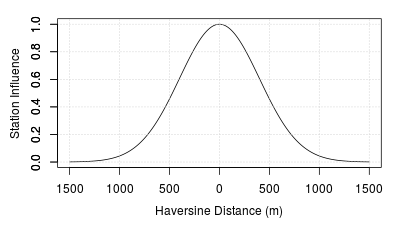
\includegraphics[width=0.60\textwidth]{influence_map}
	\caption{A station's influence function.}
	\label{fig:influence_area}
\end{figure}

Once the influence function has been placed over each subway and train station, we defined a square mesh on the map with a resolution of 100m.
For each point on this mesh we computed the influence level of the nearest station.
Finally, we computed the average influence level over all points within the same district.

\subsubsection{Reserved street parking spaces}
In areas with great daily circulation of cars and people, street parking is paid
and cars are allowed to stay a limited amount of time.
This system, called \emph{``Zona Azul''}, works in a similar fashion to parking meters in the United States.
Several of these Zona Azul parking spots are reserved for people with limited mobility,
divided in two categories: people with disabilities, and the elderly.
To be able to park in these spaces, a permit card must be obtained from the City Hall,
and it should be displayed on a car's windshield while parked.
If the proper permit is not visible, the car may be fined and towed.

In our study, we took into account these reserved places by
calculating their ``average density'' in each district,
i.e., by counting the number of reserved spots within the district and dividing by its area.
A district's score for this subfeature is obtained after grade normalization.

\subsection{Indoors - Buildings and Venues}
\label{sub:indoors}

The ideal scenario to rank indoor accessibility is to have complete information
about each and every building in the city.
At least to the extent of our knowledge, there is no such dataset available,
so the analysis was based on two sources:
the list of places granted the \emph{``Accessibility Seal''} by \emph{São Paulo City's Permanent Commission for Accessibility}~\cite{geosampa:2000},
and the \emph{guiaderodas}~\cite{guiaderodas} database, generated by their users.

Launched in 2016, guiaderodas is an accessibility guide for people with mobility difficulties.
Its mobile app lists nearby places based on user location,
allowing any person to review or consult the accessibility of venues.
It also features a text search for reviewing or checking places in any country.
The United Nations has granted it an award for being the \emph{``best initiative for inclusion \& empowerment in the world''}~\cite{belloni-gdr, yuge-gdr}.
Its database contains thousands of reviewed places in the city of São Paulo.

Users rate venues in guiaderodas by answering questions, which are presented depending on its category.
For instance, all reviews include questions about the entrance and reserved/vallet parking,
but users reviewing hotels can report the existence (or lack thereof) of accessible bedrooms,
whereas for restaurants and coffee shops they are asked about the height of tables and counters.
Not all reviews contain ratings for every criteria, as users are free to skip any question.

For each aspect, users can assign three different values, according to a color scale:
\textit{red} (bad), \textit{yellow} (average) and \textit{green} (good).
This means that the database does not contain information about accessible places only,
but also about partially or not accessible venues,
making it a valuable source of information.
Table~\ref{tab:color_scores} displays the numeric values used to map color scores into partial scores.

\begin{table}[h]
  \centering
  \begin{tabular}{llr}
    \bottomrule\addlinespace[0.3em]
    Color Rating & Score \\
    \bottomrule\addlinespace[0.3em]
    Red    & 1 \\
    Yellow & 3 \\
    Green  & 5 \\
    \addlinespace[0.3em]
    \bottomrule
  \end{tabular}
  \caption{Numeric values for crowd-sourced venue ratings.}
  \label{tab:color_scores}
\end{table}

An individual venue's score is the average of all of its user-provided ratings.
Because more than half of the districts had no data at all in the Accessibility Seal dataset,
this source was integrated into the guiaderodas database by applying maximum grade to each place listed in the collection.

The final score for this axis was the arithmetic average of all rated venues within each district.
As a consequence of geographic bias in the amount of app users,
the number of ratings in each district has high variance.
To preserve statistical relevance, districts with too few data points received no score.

\subsection{Outdoors - Topography}
\label{sub:topography}

As explained in Subsection~\ref{sub:meth-saopaulo}, Topography was the only Outdoor feature for which sufficient data was found.
It is also an important factor in assessing accessibility in urban areas.
This is a largely geographical issue, since in practice it is very difficult to change the urban topography in a macro-scale,
especially in already urbanized areas.
However, it is important to take the slope of the terrain into account in our analysis,
since very steep areas can greatly impact people with mobility restrictions.

Terrain slope is a measurement of how steep the ground surface is.
It is expressed as the percentage ratio between the \textit{rise} and \textit{run} distances, as shown in Figure~\ref{fig:slope}.
In short, the steeper the surface, the greater the slope.
The studied dataset classifies areas in four slope categories, according to Table~\ref{tab:topography}.

\vspace{0.1cm}
\begin{figure}[h]
  \centering
  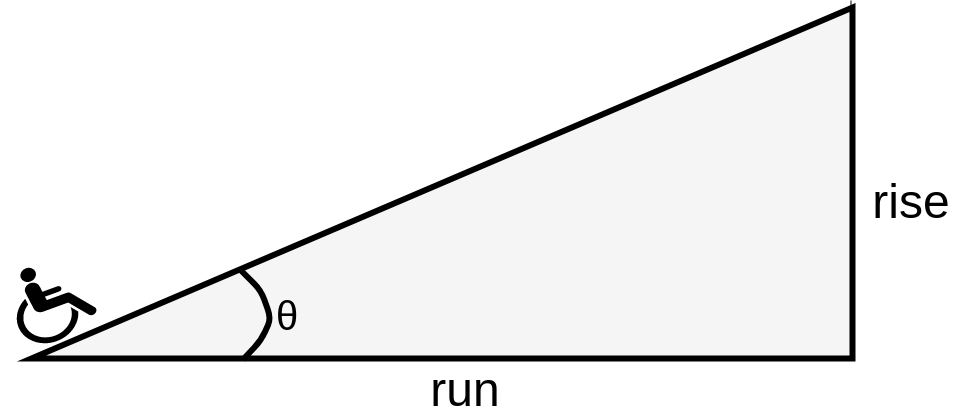
\includegraphics[width=0.50\textwidth]{slope}
  \caption{Slope measurement.}
  \label{fig:slope}
\end{figure}

\begin{table}[h]
  \small
  \centering
  \begin{tabular}{llr}
    \bottomrule\addlinespace[0.3em]
    Area & Description & Weigth \\
    \bottomrule\addlinespace[0.3em]
    1 & up to 5.0\%           & 0 \\
    2 & from 5.0\% to 25.0\%  & 5 \\
    3 & from 25.0\% to 60.0\% & 25\\
    4 & greater than 60.0\%   & 60\\
    \addlinespace[0.3em]
    \bottomrule
  \end{tabular}
  \caption{Terrain slope categories and weights.}
  \label{tab:topography}
\end{table}

We assigned a weight for each slope category, which corresponds to the lowest value of the slope range of each class. Accordingly, the topography score can be computed by a weighted average, which considers the class weight and the percentage of district's area classified in each category (equation~\ref{eq:topography_score}).

\begin{equation*}
\label{eq:topography_score}
topography\_score = \frac{0*area_1+5*area_2+25*area_3+60*area_4}{area_1+area_2+area_3+area_4}
\end{equation*}

Thus, the value of $topography\_score$ is larger for districts with bigger fractions of their area classified into steeper categories.
The final topography score is obtained after linear normalization between $0.0$ (worst performance) and $10.0$ (best).

\section{Results and Discussion}
\label{sec:results}

Table~\ref{tab:zones1} contains the total score for each city zone,
calculated as the average score of its districts.
Districts without final score were not taken into account.
A detailed table with all partial scores per district is available in the Appendix.
Figure~\ref{fig:map} presents results as a color-scaled map.

\begin{table}[h]
  \small
  \centering
  \begin{tabular}{clccccccc}
    \hline
    & \multirow{2}{*}{\textbf{Zone}}
    & \multirow{2}{*}{\textbf{Districts}}
    & \multirow{2}{*}{\textbf{Indoors}}
    & \multirow{2}{*}{\textbf{Topography}}
    & \multicolumn{3}{c}{\textbf{Mobility}}
    & \multirow{2}{*}{\textbf{Total}}
    \\[0.3ex]
    \cline{6-8}
    \multicolumn{1}{c}{}
    &  &  &  &  & \multicolumn{1}{c}{Bus} & Parking & Subway & \\[0.3ex]
    \hline
    1 & Central (C) & 8  & 6.7685   & 8.5622   & 8.3940   & 9.2626   & 6.2127   & 7.7624  \\
    2 & West    (W) & 15 & 7.3105   & 7.9030   & 6.4906   & 3.4456   & 2.4769   & 6.6239  \\
    3 & South   (S) & 33 & 6.6714   & 6.7175   & 6.0391   & 2.7474   & 1.4575   & 5.7620  \\
    4 & East    (E) & 22 & 5.5156   & 7.2920   & 6.6926   & 2.8571   & 1.5360   & 5.6242  \\
    5 & North   (N) & 18 & 5.8541   & 5.2256   & 5.5868   & 1.1833   & 0.6743   & 4.6355  \\
    \hline

  \end{tabular}
  \caption{Average district scores, per zone.}
  \label{tab:zones1}
\end{table}

\begin{figure}[ht]
  \centering
  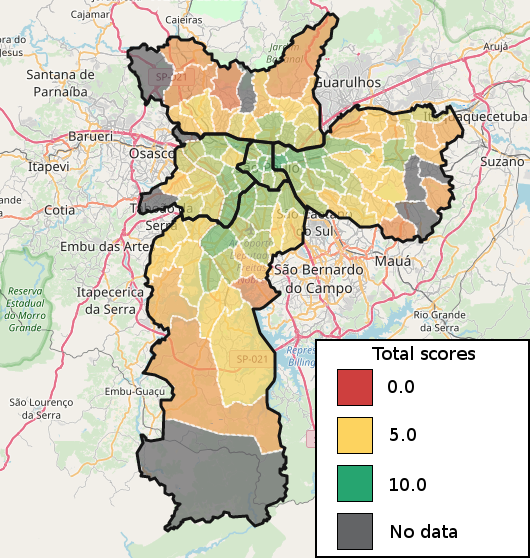
\includegraphics[width=0.75\textwidth]{map-with-legend.png}
  \caption{Final scores per district.}
  \label{fig:map}
\end{figure}

Indoor scores have a noticeably better average performance in the West Zone.
Considering that it contains many of the districts which also have better
Human Development Index (HDI) scores~\cite{atlas-idh},
this result seems to be in accordance to the qualitative perception that,
in general, its buildings have better accessibility.
As mentioned in Subsection~\ref{sub:indoors},
a geographic bias has been noticed in the database,
meaning that the distribution of rated venues is not uniform across the districts.
Therefore, it was necessary to set a minimum quantity of data points per district,
excluding ones that did not have enough data.
Such districts received no score for this axis
and are not included in Table~\ref{tab:zones1}.

Topography scores translate the peculiarity of São Paulo's geography.
The city is crossed by two major rivers, Tietê and Pinheiros,
and districts near the historical floodplains tend to have low average declivity.
Additionally, the area where the city was founded in the XVI century is also rather flat,
justifying the high average score of the Central Zone.
In the outskirts of the city, mountain ranges exist,
specially in the extreme north and south (\emph{Cantareira} and \emph{Sea} ridges, respectively).
This causes a much worse performance for districts in these areas,
which inflates the score of flatter regions.
After linear normalization, the average score of this axis was the highest
-- only 16 of the 96 districts received a grade below $5.0$.

Mobility results show the high centralization of São Paulo's public transportation infrastructure.
In general,
most of the bus routes connecting North/South and East/West zones
necessarily cross the city center.
For subway and train lines, this characteristic is even more apparent:
4 of the 5 existing subway lines go through several stops in the Central Zone,
causing a ``high density'' of stations in this area.
In São Paulo, priority parking spaces for people with disabilities and elderly citizens
only exist in streets with high daily circulation of automobiles and people.
Once again, an extreme concentration around the city center can be observed.
In fact, almost two thirds of the districts received grade zero for this aspect,
meaning that there is no reserved parking whatsoever in these parts of the city.
These facts explain the good overall performance of central districts in this feature.
Considering that the goal of the Mobility axis is to measure which areas offer more versatility for transportation,
numeric results seem to satisfactorily approximate the observed reality.

In general, results show that the districts with the best accessibility score
are strongly correlated with the central areas (specially due to Mobility factors)
and regions with higher socioeconomic indicators.
Considering that this is in accordance to the preexisting qualitative perception,
the model can be held to satisfactorily represent the observed reality.

\subsection{Limitations}
\label{sub:limitations}

It is important to highlight that due to the nature of our comparative scale,
a single isolated score does not support any kind of conclusion.
A final district's mark of $8.0$, for instance,
does tell if the district is accessible or not.
It means that, according to studied parameters and data,
it has \emph{better} accessibility than districts with lower score.

As a consequence, two separate studies with this method
yield completely independent results
that do not allow for comparisons between each other,
as grades are not akin nor interchangeable.

\subsection{Future Work}
\label{sub:future}

The evaluation criteria used in this work can still be further developed in future research
by improving both quality and quantity of analyzed data.
This includes:
expanding existing datasets,
aggregating new datasets for other subfeatures listed in Section~\ref{sec:methodology},
and taking into account the geographic distribution of people with limited mobility (i.e., \emph{``where they live''}).

Another path for improvement
is to create guidelines to compare the relevance of each feature and subfeature.
In our case study, we considered that all datasets had equal importance
and final scores were a simple arithmetic average.
For a better model of the real world,
one should be able to give greater weights to aspects considered more significant
in the generation of the final ranking.
This can be achieved by creating a group of rules to set the relevance of each subfeature.
Ideally, this rule set should be flexible and allow for proper parametrization to accommodate different realities observed in different urban zones.

Finally, this work can also serve as a starting point for the creation of an \emph{absolute} accessibility scale.
Such grading method would allow for drawing conclusions from isolated scores,
instead of the purely comparative nature of our current method.
This would solve the method's biggest drawbacks, explained in Subsection~\ref{sub:limitations}.

\section{Concluding Remarks}
\label{sec:conclusion}

In this paper we proposed a general method for
quantitatively evaluating urban areas regarding the accessibility of services and infra-structure for people with mobility difficulties.
We also presented a case study to exemplify the method's application.
Several publicly available datasets about the city of São Paulo were used to support our survey.

Obtained results seem to achieve the intended goal:
to effectively model the real world,
serving as a tool for comparative analysis of smaller regions within a greater zone
and support decision-making processes.
The method can be applied to any other city or metropolitan area,
as long as there is enough data available.
% as discussed in Section~\ref{sec:results}.

Results presented in this paper are also available as an interactive dashboard\footnote{http://interscity.org/apps/acessibilidade/}.
The webpage allows users to navigate through the city map and
select layers to visualize the overall performance in each scored axis.
By selecting a district, users can see its detailed scores and relative position for every aspect.
Featuring graphs and tables,
it is also possible to reorder districts to see the individual ranking for each feature.
The source code and data have been published under the MIT License\footnote{https://github.com/jbarguil/free-wheels}.

\begin{comment}
This work also serves as an evidence of how the introduction of smart cities technology,
in particular the availability of open data,
can foster initiatives in order to bring benefits
to the public,
aimed at raising the quality of life,
improving transparency in the use of city resources,
and providing tools for better public management.
\end{comment}

\section{Acknowledgements}
\label{sec:ack}

This research was conducted in the summer course of \textit{Advanced Topics in Smart Cities} at the Institute of Mathematics and Statistics, University of São Paulo (IME-USP), Brazil.
Our special thanks go to prof. Antonio Deusany de Carvalho Junior, Jairo Marques,
and São Paulo's Secretariat for People With Disabilities,
who have all contributed with several insights for this work.
We would also like to thank the public and private organizations which provided the databases used in this research: GeoSampa, SPTrans, Scipopulis and guiaderodas.

\bibliographystyle{sbc}
\bibliography{sbc-template}

\newpage
\section*{Appendix}
\label{sec:appendix}

Table \ref{tab:results} displays each district's final score for each analysed aspect.

% Table with districts' scores.
\footnotesize
\begin{longtable}[c]{c|lccccc|c}
% Table Header.
\hline
\multicolumn{1}{c}{}    % Hack to hide the vertical bar.
& \multirow{2}{*}{\textbf{District (Zone)}}
& \multirow{2}{*}{\textbf{Indoors}}
& \multirow{2}{*}{\textbf{Topography}}
& \multicolumn{3}{|c|}{\textbf{Mobility}}
& \multirow{2}{*}{\textbf{Total}}
\\
\cline{5-7}
\multicolumn{1}{c}{}    % Hack to hide the vertical bar.
&  &  &  & \multicolumn{1}{|c}{\textbf{Bus}} & \textbf{Parking} & \textbf{Subway} & \\
\hline
\endfirsthead

% Table header that is repeated in all pages.
% \multicolumn commands hacks to hide vertical bars.
\multicolumn{1}{c}{\textbf{}} & \textbf{District (Zone)} & \textbf{Indoors} & \textbf{Topography} & \textbf{Bus} & \textbf{Parking} & \multicolumn{1}{c}{\textbf{Subway}} & \textbf{Total} \\
\hline
\endhead

1   & Brás               (E) & 8.9678   & 10.0000  & 8.2026   & 9.9478   & 7.0600   & 9.1238  \\
2   & República          (C) & 7.1981   & 9.0139   & 9.5931   & 10.0000  & 9.1583   & 8.5986  \\
3   & Sé                 (C) & 6.5024   & 8.8656   & 10.0000  & 9.8820   & 10.0000  & 8.4429  \\
4   & Barra Funda        (W) & 8.8366   & 9.6899   & 7.4515   & 7.8462   & 4.1212   & 8.3331  \\
5   & Belém              (E) & 8.5266   & 9.6832   & 7.8384   & 8.2982   & 3.0432   & 8.2010  \\
6   & Santo Amaro        (S) & 9.6214   & 9.0258   & 7.9655   & 6.3589   & 3.4356   & 8.1891  \\
7   & Bom Retiro         (C) & 7.1954   & 9.8676   & 7.3120   & 9.5125   & 5.6605   & 8.1860  \\
8   & Itaim Bibi         (W) & 8.4577   & 9.8279   & 7.1126   & 9.1278   & 2.4399   & 8.1708  \\
9   & Bela Vista         (C) & 8.6106   & 7.1390   & 8.8633   & 9.4396   & 6.8864   & 8.0487  \\
10  & Tatuapé            (E) & 8.2186   & 9.4290   & 7.5035   & 8.0805   & 3.6897   & 8.0240  \\
11  & Moema              (S) & 8.8442   & 9.6061   & 7.6009   & 9.1940   & 0.0544   & 8.0222  \\
12  & Pinheiros          (W) & 6.6238   & 9.0581   & 7.8187   & 9.1627   & 5.8688   & 7.7662  \\
13  & Jardim Paulista    (W) & 7.1239   & 8.7706   & 8.0134   & 9.6033   & 3.7969   & 7.6774  \\
14  & Consolação         (C) & 7.6892   & 7.7326   & 7.7919   & 9.9017   & 5.0511   & 7.6678  \\
15  & Penha              (E) & 8.6992   & 7.8027   & 7.4625   & 7.5535   & 2.7631   & 7.4761  \\
16  & Vila Mariana       (S) & 6.9935   & 7.6956   & 7.6589   & 9.0050   & 6.2814   & 7.4459  \\
17  & Lapa               (W) & 6.7660   & 8.6128   & 7.0249   & 8.3909   & 3.7455   & 7.2553  \\
18  & Socorro            (S) & 7.1976   & 9.4562   & 6.9439   & 6.5742   & 1.5179   & 7.2219  \\
19  & Mooca              (E) & 6.8723   & 8.7969   & 6.7616   & 8.0967   & 3.0615   & 7.2142  \\
20  & Santana            (N) & 7.1155   & 8.2743   & 7.0345   & 7.6163   & 3.8040   & 7.1804  \\
21  & Itaquera           (E) & 8.8604   & 7.0979   & 7.4250   & 7.0185   & 2.2466   & 7.1739  \\
22  & Santa Cecília      (C) & 4.6467   & 9.4983   & 7.8063   & 8.7151   & 5.4471   & 7.1559  \\
23  & Ipiranga           (S) & 6.5856   & 8.8110   & 6.7358   & 7.6092   & 3.7936   & 7.1476  \\
24  & Liberdade          (C) & 6.5584   & 7.5215   & 8.1285   & 8.4459   & 5.2268   & 7.1157  \\
25  & Saúde              (S) & 7.0454   & 7.8611   & 6.7112   & 7.8024   & 4.6935   & 7.1030  \\
26  & Pari               (E) & 4.7934   & 9.9685   & 7.3663   & 9.6505   & 1.4944   & 6.9774  \\
27  & Vila Formosa       (E) & 8.8154   & 7.1578   & 6.7982   & 7.8944   & 0.0096   & 6.9580  \\
28  & Carrão             (E) & 9.9655   & 8.5261   & 6.8991   & 0.0000   & 0.2392   & 6.9570  \\
29  & Água Rasa          (E) & 8.5841   & 7.7545   & 6.5662   & 5.9307   & 0.8339   & 6.9274  \\
30  & Cambuci            (C) & 5.7474   & 8.8590   & 7.6572   & 8.2043   & 2.2716   & 6.8836  \\
31  & Jabaquara          (S) & 8.6557   & 6.8783   & 6.1742   & 6.4582   & 2.2969   & 6.8368  \\
32  & Campo Belo         (S) & 7.0753   & 8.4275   & 7.5145   & 7.4400   & 0.0305   & 6.8326  \\
33  & Vila Guilherme     (N) & 8.9332   & 8.8822   & 6.7286   & 0.0000   & 0.4648   & 6.7377  \\
34  & Vila Prudente      (E) & 6.1092   & 8.1287   & 6.7755   & 7.2929   & 3.3173   & 6.6777  \\
35  & Alto de Pinheiros  (W) & 8.4855   & 8.4076   & 5.8826   & 0.0000   & 2.5676   & 6.5699  \\
36  & Vila Leopoldina    (W) & 6.5186   & 9.5003   & 6.3147   & 0.0000   & 4.7236   & 6.5661  \\
37  & Campo Grande       (S) & 8.6704   & 8.2941   & 6.8046   & 0.0000   & 1.0923   & 6.5323  \\
38  & Aricanduva         (E) & 8.0661   & 7.9893   & 7.6046   & 0.0000   & 0.0000   & 6.1968  \\
39  & Vila Sônia         (W) & 10.0000  & 6.3099   & 6.2694   & 0.0000   & 0.0000   & 6.1333  \\
40  & Vila Maria         (N) & 7.5469   & 8.8271   & 5.6808   & 0.0000   & 0.0004   & 6.0892  \\
41  & Jaguaré            (W) & 7.6243   & 7.6522   & 5.5822   & 0.0000   & 2.7983   & 6.0233  \\
42  & Jardim Helena      (E) & 5.2923   & 9.9521   & 4.5307   & 0.0000   & 2.8703   & 5.9038  \\
43  & São Miguel         (E) & 3.4040   & 8.4264   & 7.4120   & 7.9429   & 2.0583   & 5.8783  \\
44  & Morumbi            (W) & 8.3303   & 6.4307   & 5.9870   & 0.0000   & 2.2985   & 5.8409  \\
45  & Limão              (N) & 6.9449   & 7.8858   & 6.7339   & 0.0000   & 0.0017   & 5.6920  \\
46  & Butantã            (W) & 6.4648   & 7.7981   & 6.4196   & 0.0000   & 1.9135   & 5.6802  \\
47  & Vila Medeiros      (N) & 3.0371   & 8.7564   & 6.1972   & 7.2970   & 0.0037   & 5.4309  \\
48  & Sapopemba          (E) & 7.7553   & 6.2571   & 6.5774   & 0.0000   & 0.0000   & 5.4016  \\
49  & Perdizes           (W) & 4.0185   & 6.5731   & 6.7239   & 7.5531   & 2.5578   & 5.4011  \\
50  & Campo Limpo        (S) & 8.2077   & 5.2280   & 6.6516   & 0.0000   & 1.4334   & 5.3769  \\
51  & Vila Andrade       (S) & 8.8096   & 4.4472   & 6.4087   & 0.0000   & 2.2129   & 5.3769  \\
52  & Sacomã             (S) & 6.7308   & 7.3734   & 5.4297   & 0.0000   & 0.2303   & 5.3303  \\
53  & Jardim São Luis    (S) & 6.7711   & 6.5665   & 6.4659   & 0.0000   & 0.9361   & 5.2683  \\
54  & Vila Matilde       (E) & 5.2948   & 7.3066   & 6.1868   & 0.0000   & 3.4023   & 5.2659  \\
55  & Pirituba           (N) & 8.2185   & 4.5260   & 5.6152   & 0.0000   & 2.7645   & 5.1792  \\
56  & Grajaú             (S) & 7.1423   & 6.7264   & 4.8120   & 0.0000   & 0.1006   & 5.1688  \\
57  & Casa Verde         (N) & 5.8679   & 7.2872   & 6.6526   & 0.0000   & 0.0060   & 5.1249  \\
58  & Cursino            (S) & 6.1061   & 7.0124   & 5.6791   & 0.0000   & 0.8457   & 5.0978  \\
59  & Cidade Dutra       (S) & 5.2370   & 7.4058   & 6.1133   & 0.0000   & 1.5598   & 5.0668  \\
60  & Cidade Líder       (E) & 7.4790   & 5.4505   & 6.6487   & 0.0000   & 0.0249   & 5.0514  \\
61  & Parque do Carmo    (E) & 8.4209   & 4.6188   & 5.9003   & 0.0000   & 0.0004   & 5.0022  \\
62  & Artur Alvim        (E) & 3.9048   & 7.4022   & 7.4009   & 0.0000   & 3.2886   & 4.9567  \\
63  & Tucuruvi           (N) & 5.1847   & 6.6105   & 6.3188   & 0.0000   & 2.7969   & 4.9446  \\
64  & Capão Redondo      (S) & 6.4939   & 5.1885   & 6.8695   & 0.0000   & 1.5413   & 4.8287  \\
65  & São Mateus         (E) & 4.8286   & 7.1285   & 6.9755   & 0.0000   & 0.0000   & 4.7607  \\
66  & Ermelino Matarazzo (E) & 3.6630   & 7.5800   & 6.2494   & 0.0000   & 2.7472   & 4.7473  \\
67  & Rio Pequeno        (W) & 5.7869   & 6.3629   & 5.7922   & 0.0000   & 0.0000   & 4.6935  \\
68  & São Lucas          (E) & 3.6014   & 7.6410   & 6.6706   & 0.0000   & 1.0142   & 4.6014  \\
69  & Jaçanã             (N) & 4.3604   & 6.7453   & 6.3728   & 0.0000   & 0.0000   & 4.4100  \\
70  & São Domingos       (N) & 5.5300   & 5.9093   & 5.0466   & 0.0000   & 0.0965   & 4.3846  \\
71  & Cidade Ademar      (S) & 5.0348   & 5.8003   & 6.6585   & 0.0000   & 0.0000   & 4.3515  \\
72  & Mandaqui           (N) & 6.6330   & 3.7312   & 5.8140   & 0.0000   & 0.0002   & 4.1007  \\
73  & Ponte Rasa         (E) & 1.7925   & 7.8219   & 7.9363   & 0.0000   & 0.0109   & 4.0878  \\
74  & Vila Jacuí         (E) & 2.1885   & 7.6070   & 7.2833   & 0.0000   & 0.0042   & 4.0749  \\
75  & Freguesia do Ó     (N) & 3.8291   & 6.2649   & 6.2879   & 0.0000   & 0.0321   & 4.0669  \\
76  & Lajeado            (E) & 2.8120   & 6.8612   & 6.4046   & 0.0000   & 1.1550   & 4.0644  \\
77  & Jardim Ângela      (S) & 5.0924   & 4.9216   & 5.0890   & 0.0000   & 0.0000   & 3.9034  \\
78  & Cangaíba           (E) & 1.0360   & 8.2365   & 5.4781   & 0.0000   & 1.7364   & 3.8924  \\
79  & Itaim Paulista     (E) & 1.0730   & 7.4432   & 5.7508   & 0.0000   & 1.3071   & 3.6229  \\
80  & Vila Curuçá        (E) & 0.0000   & 8.0094   & 6.9277   & 0.0000   & 1.0697   & 3.5584  \\
81  & Parelheiros        (S) & 3.7818   & 4.8389   & 3.5451   & 0.0000   & 0.0000   & 3.2675  \\
82  & Cidade Tiradentes  (E) & 4.0755   & 3.7278   & 5.8739   & 0.0000   & 0.0000   & 3.2538  \\
83  & Perus              (N) & 5.8214   & 1.9817   & 3.5030   & 0.0000   & 0.7924   & 3.0783  \\
84  & Tremembé           (N) & 7.3223   & 0.3945   & 3.6003   & 0.0000   & 0.0000   & 2.9723  \\
85  & Jaraguá            (N) & 4.2134   & 2.0122   & 4.8130   & 0.0000   & 1.3747   & 2.7627  \\
86  & São Rafael         (E) & 2.3680   & 4.0718   & 4.9297   & 0.0000   & 0.0000   & 2.6943  \\
87  & Pedreira           (S) & 0.0025   & 6.2212   & 5.0272   & 0.0000   & 0.0092   & 2.6342  \\
88  & Brasilândia        (N) & 3.1080   & 1.0752   & 5.5746   & 0.0000   & 0.0000   & 2.0138  \\
-   & Anhanguera         (N) & -        & 1.8401   & 2.2314   & 0.0000   & 0.0000   & -       \\
-   & Cachoeirinha       (N) & -        & 3.0568   & 6.3568   & 6.3860   & 0.0000   & -       \\
-   & Guaianases         (E) & -        & 5.3328   & 6.7099   & 6.5771   & 1.1588   & -       \\
-   & Iguatemi           (E) & -        & 2.1634   & 5.2813   & 0.0000   & 0.0000   & -       \\
-   & Jaguara            (W) & -        & 8.0224   & 5.8091   & 0.0000   & 0.3225   & -       \\
-   & José Bonifácio     (E) & -        & 5.2635   & 6.5253   & 0.0000   & 1.0798   & -       \\
-   & Marsilac           (S) & -        & 0.0000   & 0.0000   & 0.0000   & 0.0000   & -       \\
-   & Raposo Tavares     (W) & -        & 5.5289   & 5.1573   & 0.0000   & 0.0000   & -       \\

\caption{Final scores by district.}
\label{tab:results}
\end{longtable}
\normalsize

\end{document}
